Tal como se menciona en el Capitulo \ref{cap:mats}, los circuitos integrados utilizados para la implementación de la comunicación USB, estos son el controlador FX2LP de Cypress y el FPGA Spartan VI de Xilinx, vienen incorporados en sendas placas de desarrollo. Para la conexión eléctrica de estos dos chips, se desarrolla una placa de interconexión, es decir, un circuito impreso (PCB, del ingles {\it Printed Circuit Board}) que sirve para conectar en forma eléctrica dos o más dispositivos. Esto brinda una conexión mucho más robusta, compacta y prolija que si fuese realizada mediante cables o alambres.

\begin{figure}[ht]
	\centering
	\begin{subfigure}[t]{0.45\textwidth}
		\centering
		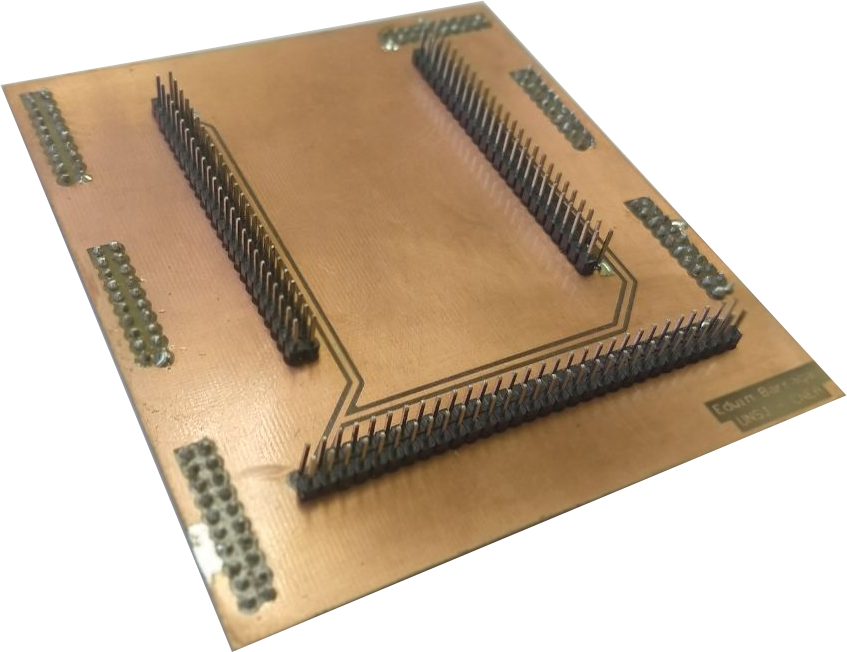
\includegraphics[width=\textwidth]{pcbv1anv}
		\caption*{Anverso}
	\end{subfigure}
	\begin{subfigure}[t]{0.45\textwidth}
		\centering
		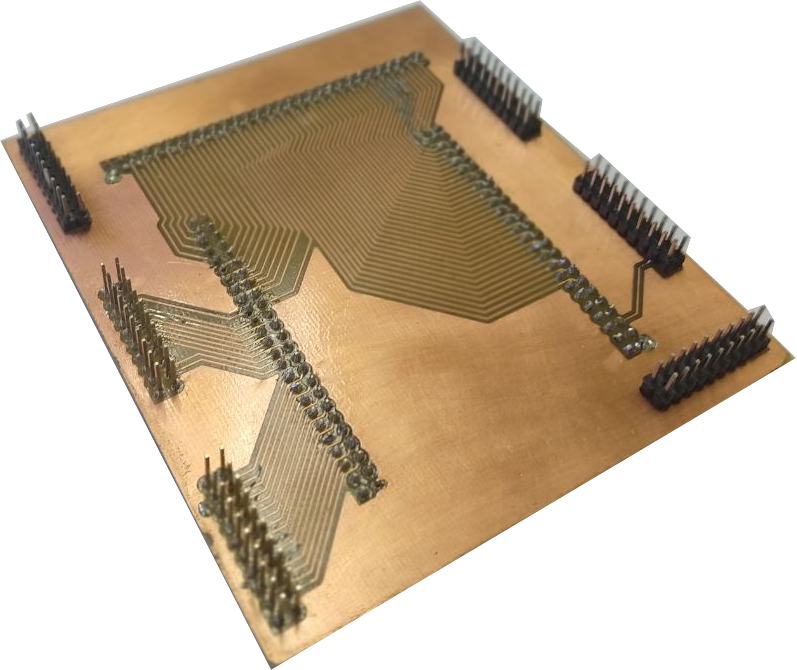
\includegraphics[width=\textwidth]{pcbv1rev}
		\caption*{Reverso}
	\end{subfigure}
	\caption{Versión 1 de la placa de interconexión}
	\label{fpga:pcb:v1}
\end{figure}

El desarrollo de la placa de interconexión, necesitó de tres versiones para obtener un correcto funcionamiento. La versión número 1, la cual se observa en la Figura \ref{fpga:pcb:v1}, presenta un problema de contacto eléctrico entre sus dos caras conductoras, debido a no se contaba con la tecnología suficiente para realizar la metalización de los agujeros que conducen la señal de un lado al otro del circuito impreso durante el proceso de fabricación. Por otro lado, en la etapa de montaje, el alumno confunde los pines que debe ser colocados, ya que el reverso necesita pines hembra en lugar de pines macho.

\begin{figure}[ht]
	\centering
	\begin{subfigure}[t]{0.45\textwidth}
		\centering
		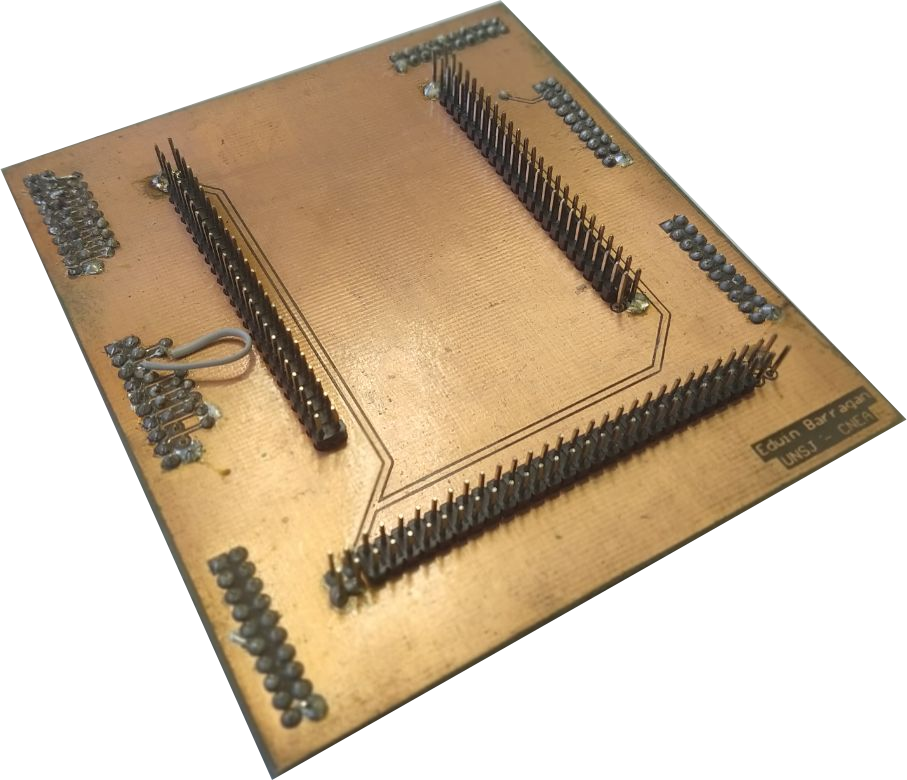
\includegraphics[width=\textwidth]{pcbv2anv}
		\caption*{Anverso}
	\end{subfigure}
	\begin{subfigure}[t]{0.45\textwidth}
		\centering
		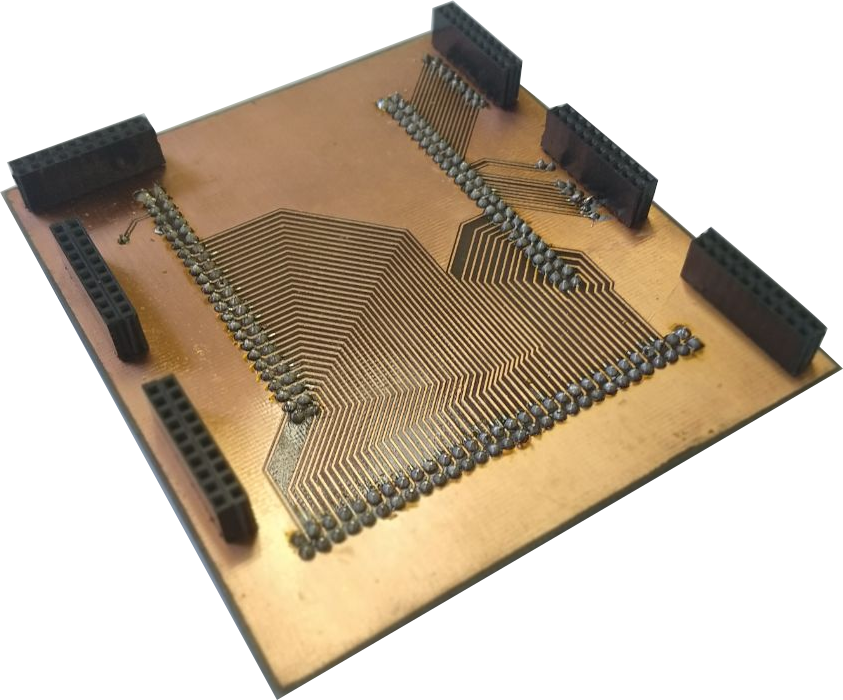
\includegraphics[width=\textwidth]{pcbv2rev}
		\caption*{Reverso}
	\end{subfigure}
	\caption{Versión 2 de la placa de interconexión}
	\label{fpga:pcb:v2}
\end{figure}

Se realiza una segunda versión, la que se observa en la Figura \ref{fpga:pcb:v2}. A este PCB se le incorporan vías pasantes para poder conectar las distintas pistas que recorren el circuito mediante la soldadura de alambres, lo que soluciona el problema de conexión eléctrica. En esta placa se tiene mayor cuidado en la etapa de montaje de los pines. Sin embargo, durante la revisión de los pines se encuentra un defecto en el puerto asignado a la señal de reloj, la cual posee un terminal en un pin que no se encuentra disponible. Esto obliga a la implementación de la comunicación del presente trabajo de forma asíncrona.

Otro defecto que presenta la versión 2 de la placa de interconexión es la inexistencia de un punto para soldadura, que se ocasiona al momento del perforado del impreso. Esto obliga a realizar una conexión mediante un pequeño cable, el cual se puede observar en el anverso de la Figura \ref{fpga:pcb:v2}.

\begin{figure}[ht]
	\centering
	\begin{subfigure}[t]{0.45\textwidth}
		\centering
		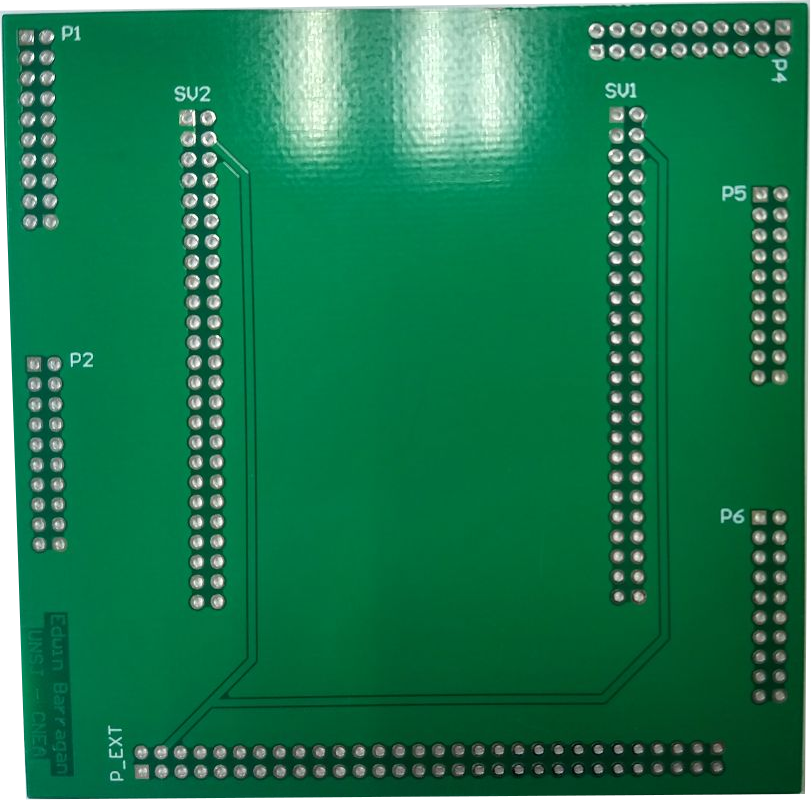
\includegraphics[width=\textwidth]{pcbv3anv}
		\caption*{Anverso}
	\end{subfigure}
	\begin{subfigure}[t]{0.45\textwidth}
		\centering
		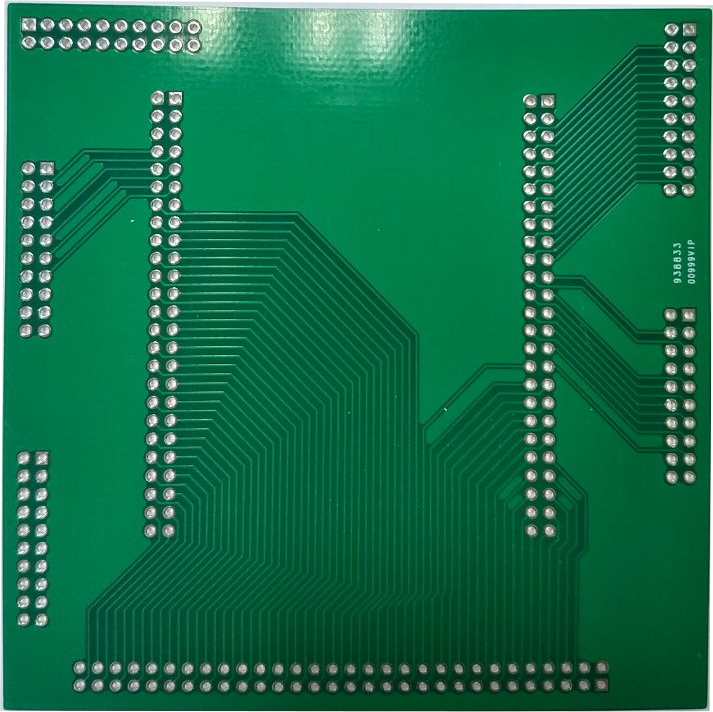
\includegraphics[width=\textwidth]{pcbv3rev}
		\caption*{Reverso}
	\end{subfigure}
	\caption{Versión 3 de la placa de interconexión}
	\label{fpga:pcb:v3}
\end{figure}

Finalmente, se decide rehacer el circuito de conexión en una tercera versión y solicitar su fabricación en una empresa especializada en la manufactura de PCB para prototipo, radicada en China. En esta versión, fue redirigida la línea de conexión defectuosa, lo que permite conectar las fuentes de reloj e implementar una comunicación síncrónica. Esto no fue realizado al momento de la escritura del presente informe, aunque se espera su implementación en trabajos futuros. Además, debido a restricciones en el proceso de fabricación, se debe redimensionar el PCB y hacerlo más compacto.

Gracias a la mejora que brinda la empresa en el proceso de fabricación, se eliminan las conexiones entre las dos caras del impreso mediante la soldadura de alambre y se cambian por agujeros metalizados. Además, se incorporaron conexiones adicionales entre el controlador y el FPGA. Esto permite utilizar el $\mu$C 8051 incorporado al controlador FX2LP para realizar tareas adicionales, junto al FPGA. Se adjunta en el Anexo \ref{an:pcb} un plano esquemático con las conexiones de la versión 3 del circuito impreso. elaborado.